\documentclass[a4paper, 12pt]{article}%тип документа

%отступы
\usepackage[left=2cm,right=2cm,top=2cm,bottom=3cm,bindingoffset=0cm]{geometry}

%Русский язык
\usepackage[T2A]{fontenc} %кодировка
\usepackage[utf8]{inputenc} %кодировка исходного кода
\usepackage[english,russian]{babel} %локализация и переносы

%Вставка картинок
\usepackage{wrapfig}
\usepackage{graphicx}
\graphicspath{{pictures/}}
\DeclareGraphicsExtensions{.pdf,.png,.jpg}

%оглавление
\usepackage{titlesec}
\titlespacing{\chapter}{0pt}{-30pt}{12pt}
\titlespacing{\section}{\parindent}{5mm}{5mm}
\titlespacing{\subsection}{\parindent}{5mm}{5mm}
\usepackage{setspace}

%Графики
\usepackage{multirow}
\usepackage{pgfplots}
\pgfplotsset{compat=1.9}

%Математика
\usepackage{amsmath, amsfonts, amssymb, amsthm, mathtools}

%Заголовок
\author{Валеев Рауф Раушанович \\
группа 825}
\date{}
\title{\textbf{Работа 4.3.1\\Дифракции Френеля и Фраунгофера}}
\newtheorem{task}{Задача}
\begin{document}
\maketitle
\textbf{Цель работы}: исследовать являения дифракции Френеля и Фраунгофера на щели, изучить влияние дифракции на разрешающую способность оптических инструментов.


\textbf{В работе используются}: оптическая скамья, ртутная лампа, монохроматор, щели с регулируемой шириной, рамка с вертикальной нитью, двойная щель, микроскоп на поперечных салазках с микрометрическим винтом, зрительная труба.
\section{Дифракция Френеля}
\subsection*{Установка}
\begin{figure}[h]
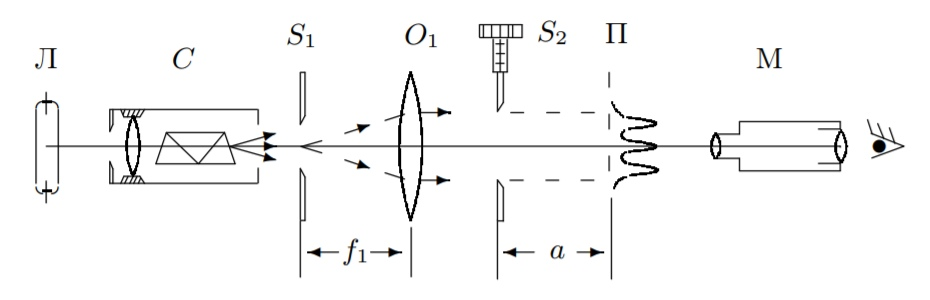
\includegraphics[width=0.7\textwidth]{7.jpg}
\centering
\caption{Схема установки.}
\end{figure}
Схема установки представлена на Рис. 1.\\
\subsection*{Теория}
Распределение интенсивности света в плоскости П рассчитаем с помощью зон Френеля. При освещении $S_2$ параллельным пучком лучей (плоская зона) зоны Френеля представляют собой плоскости, параллельные краям щели. Результирующая амплитуда в точке наблюдения определеяется суперпозицией колебаний от тех зон Френеля, которые не перекрыты створками щели. Графическое определение результирующей амплитуды производится с помощью векторной диаграммы -- спирали Корню. Суммарная ширина $m$ зон Френеля $z_m$ определяется соотношение
\begin{equation}
z_m = \sqrt{am\lambda},
\end{equation}
где $a$ -- расстояние от щели до плоскости П. Вид наблюдаемой картины определяется \textit{числом Френеля} $\Phi$:
$$
\Phi^2 = \dfrac{D}{\sqrt{a\lambda}}
$$
-- число зон Френеля, которые укладываются в ширине щели $D$. $p = \frac{1}{\Phi^2}$ называется \textit{волновым параметром}. 
\subsection*{Ход работы}
\begin{enumerate}
\item Соберем и настроим экспериментальную установку. 
\item Постепенно отодвигая микроскоп от $S_2$, отметим положение, при котором на фоне щели видна одна тёмная полоса. Смещение от начального положения даёт $a$.
\item Измеряем ширину $D$ щели $S_2$ с помощью микрометрического винта и поперечных салазок микроскопа и 
\[D_{micro} = (2,855 \pm 0,005) \cdot 10^{-4} \text{м}\]
\[D_{shel} = (2,75 \pm 0,05) \cdot 10^{-4} \text{м}\]
В данных, написанных выше, берем погрешность, равную половине цены деления шкалы, то есть в случае микрометрического винта: $0,001/2$, а в случае салазок микроскопа: $0,01/2$.
\item Проследим за изменением количества полос при изменении расстояния $a$. Принимая $x_0 = 46,8$ см, запишем все данные, которые мы получили, и из формулы $(1)$ получим $2z_m$, сравним из с $D$ и построим это все на графике. При расчетах используются $\lambda = 576,96$ нм.

\begin{table}[h]
\begin{center}
\begin{tabular}{|c|c|c|c|c|c|}
\hline
количество полос m & $x$, см & $\delta x$, см & $a_m$, см & $2z_m$, мкм & $\delta(2z_m)$, мкм \\ \hline
1                  & 44,20    & 0,05           & 2,6       & 245         & 9                   \\ \hline
2                  & 45,00      & 0,05            & 1,8       & 289         & 16                  \\ \hline
3                  & 45,60    & 0,05            & 1,2       & 290         & 20                  \\ \hline
4                  & 465      & 0,05            & 0,8       & 270         & 30                  \\ \hline
5                  & 46,15    & 0,05           & 0,7       & 280         & 40                  \\ \hline
6                  & 46,25    & 0,05            & 0,6       & 290         & 40                  \\ \hline
\end{tabular}
\caption{Зависимость расстояния от щели до плоскости наблюдения от числа темных полос.}
\end{center}
\end{table}

Погрешности в таблице выше получаются для $x$ из половины цены деления поперечных салазок микроскопа (было описано в пункте 3), а для $z_m$ из почленного дифференцирования формулы $(1)$, а именно погрешность для $z_m$ равна 
\[ \delta(2 z_m) = 2	z_m \cdot \sqrt{\left(\dfrac{\partial \left( 2\sqrt{a_mm\lambda} \right)}{\partial a_m}\right)^{2} \sigma_{a_m}^2} = 2 z_m \sqrt{\dfrac{m \lambda}{a_m}} \sigma_{a_m}\]
А если вспомнить, что $z_m = \sqrt{a_m m \lambda}$, то формула погрешности примет вид, который использовался для подсчета погрешности в таблице:
\[\delta(2z_m) = 2 m \lambda \sigma_{a_m}\]
Усреднив $2z_m$ мы получим ширину щели $D$, погрешность для нее считается по формуле 
\[\delta D_{mid} = \dfrac{1}{\sqrt{n(n-1)}} \cdot \sqrt{\sum\limits_{i = 1}^n\left(D_i - D_{mid}\right)^2}\]
и итоговая погрешность 
\[\delta D = D \cdot \sqrt{\sigma^2 (D)_{mid} + (\delta D/D)^2}\]
Все это будет показано численно в выводе.
\begin{figure}[h!]
\begin{center}
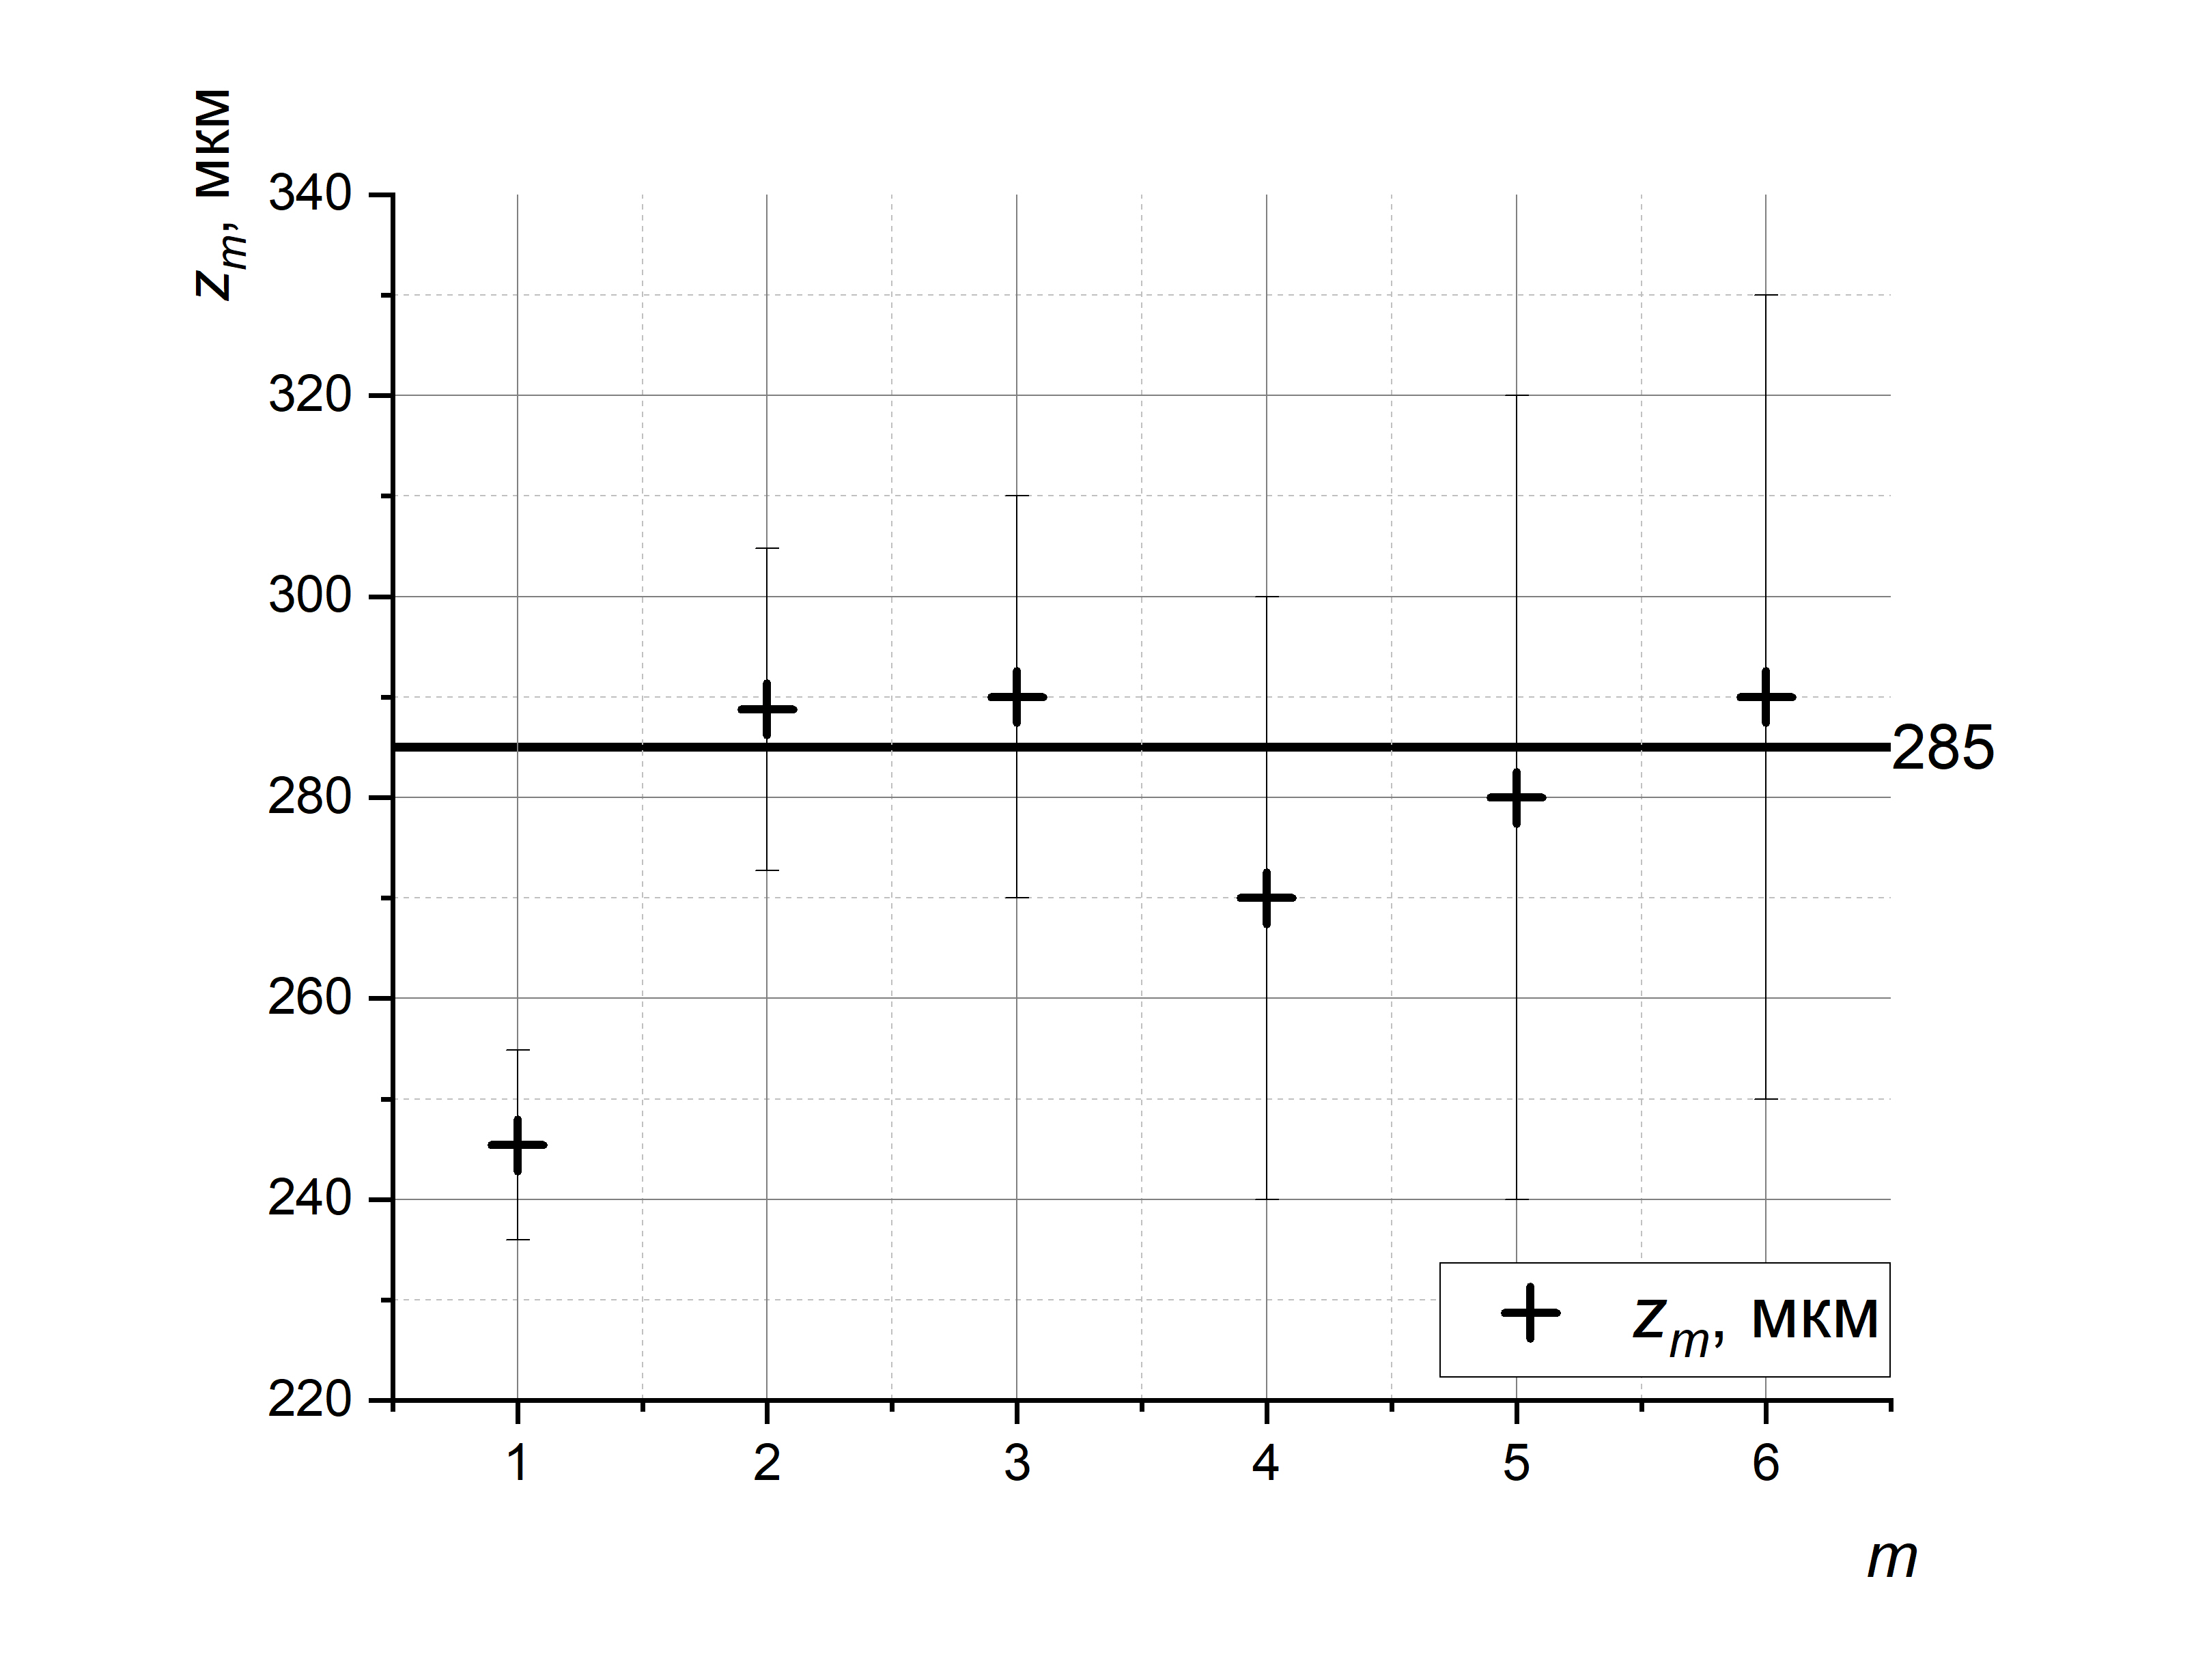
\includegraphics[width = 0.8\textwidth]{8.jpg}
\caption{Визуализация данных, полученных в пункте А}
\end{center}
\end{figure}
\end{enumerate}
\section{Дифракция Фраунгофера на щели}
\subsection*{Теория}
\begin{wrapfigure}{r}{0.5\textwidth}
  \begin{center}
    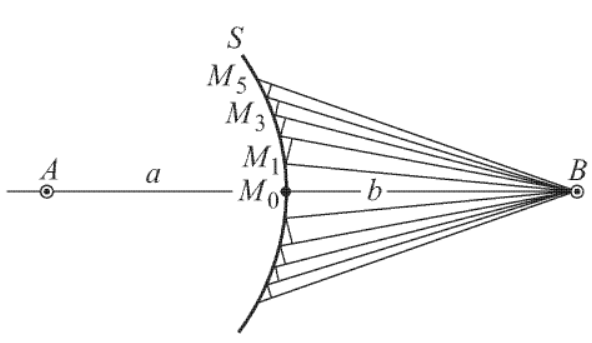
\includegraphics[width = 0.4\textwidth]{2.png}
  \end{center}
  \caption{Построение зон Френеля}
\end{wrapfigure}
Для выкладок ниже нам потребуется знать \textit{принцип Гюйгенса-Френеля}. Он формулируется следующим образом 

\textit{Каждый элемент волнового фронта можно рассматривать как центр  вторичного возмущения, порождающего вторичные сферические волны, а результирующее световое поле  в каждой точке пространства будет определяться интерференцией этих волн.}

Теперь рассмотрим первое применение этого принципа, получившее название \textit{метод зон Френеля}

Для этого рассмотрим действие световой волны действующей из точки $A$ в какой-то точке $B$.

В этом случае можно, взяв точку $M_0$ в качестве центра (см. рис. 1), построить ряд концентрических сфер, радиусы которых начинаются с $b$ и увеличиваются каждый раз на половину длины волны $\lambda/2$. При пересечении с плоским фронтом волны $F$ эти сферы дадут концентрические окружности. Таким образом, на фронте волны появятся кольцевые зоны (зоны Френеля) с радиусами $r_1, r_2$ и т. д.

Из геометрических соображений посчитав, можно получить, что 
\begin{equation}
r_i = i \sqrt{a \lambda}
\end{equation}	
Введем так же обозначение: \textit{число Френеля}
\begin{equation}
\Phi^2 = \dfrac{D}{\sqrt{a\lambda}}
\end{equation}
\begin{wrapfigure}{r}{0.5\textwidth}
  \begin{center}
    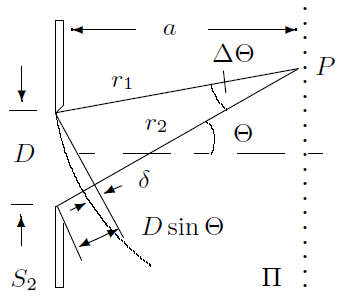
\includegraphics[width = 0.35\textwidth]{1.png}
  \end{center}
  \caption{К фазовым соотношениям при дифракции Фраунгофера}
\end{wrapfigure}
В этом пункте рассмотрим дифракцию, когда ширина щели становится значительно меньше ширины первой зоны Френеля, т.е. если 
\begin{equation}
D \ll\sqrt{a \lambda} 
\end{equation}	
Это условие всегда выполняется при достаточно большом $a$. В этом случае говорят, что \textit{дифракция Фраунгофера}. При выполнении пункта $(2)$ у нас заметно упрощаются фазовые соотношения, что поясняет рис. 2, в итоге с хорошим приближением можно считать, что разность хода между соседними лучами равна 
\begin{equation}
\Delta = r_2 - r_1 \approx D \sin \theta \approx D \cdot \theta
\end{equation}
Здесь предполагается, что $\theta$ достаточно мал.

\subsection*{Схема установки}
Дифракцию Фраунгофера можно наблюдать на подобной установке 

\begin{figure}[h]
\begin{center}
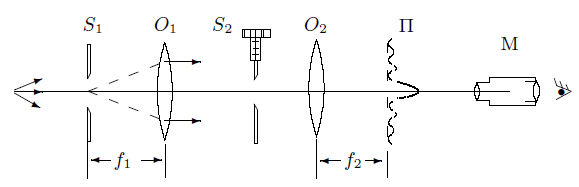
\includegraphics[width = 0.7\textwidth]{3.png}
\caption{Схема установки для пункта 2}
\end{center}
\end{figure}

Объектив здесь нужен для удобства, так как неудобно работать с очень узкими щелями. Дифракционная картина здесь наблюдается в фокальной плоскости объектива $O_2$. 

Посчитав легко определить угловую координату любой темной полосы:
\begin{equation}
\theta_m = \frac{m \lambda}{D}
\end{equation}
И расстояние от центра соответственно 
\begin{equation}
X_m = f_2m\frac{\lambda}{D}
\end{equation}
\subsection*{Ход работы}
Для начала запишем фокусные расстояния линз: $F_1 = 9$ см, $F_2 = 10,8$ см. Ширина щели $D = (395 \pm 5)$ мкм. 
Такая погрешность, потому что опять таки берем половину цены деления.
\begin{enumerate}
\item Добавим линзу $O_2$ и настроим микроскоп на фокальную плоскость. Затем подберём ширину щели, для получения дифракции.
\item Измерим $X_m$ нескольких минимумов и запишем все в таблицу и построим график.

\begin{table}[h]
\begin{center}
\begin{tabular}{|c|c|c|c|c|}
\hline
номер минимума m & $X_m$, мм & $\delta X_m$, мм & $D$, мм & $\delta D$, мм \\ \hline
1                & 0,16      & 0,005             & 0,39    & 0,03          \\ \hline
2                & 0,34      & 0,005             & 0,37    & 0,03           \\ \hline
3                & 0,46      & 0,005             & 0,40    & 0,03           \\ \hline
4                & 0,64      & 0,005             & 0,39    & 0,03           \\ \hline
-1               & -0,16     & 0,005             & 0,39    & 0,03           \\ \hline
-2               & -0,34     & 0,005             & 0,37    & 0,03           \\ \hline
-3               & -0,46     & 0,005             & 0,40    & 0,03           \\ \hline
-4               & -0,64     & 0,005             & 0,39    & 0,03           \\ \hline
\end{tabular}
\caption{Данные, измеренные в пункте Б}
\end{center}
\end{table}

Для $X_m$ такая погрешность, поскольку брали половину цены деления. В данной таблице $D$ мы находили из формулы $(7)$, соответственно погрешность мы считаем по формуле
\[\delta D = D \cdot \sqrt{ \left(\dfrac{\partial \left(f_2 m \frac{\lambda}{X_m}\right)}{\partial X_m}\right)^{2} \cdot \sigma_{X_m}^2} = D \cdot\dfrac{f_2m \lambda}{X_m^2} \cdot \sigma_{X_m}\]
Опять таки можем подставить $D$: 

\[\delta D = \dfrac{f_2^2m^2\lambda^2}{X_m^3} \sigma_{X_m} = \dfrac{D^2}{X_m} \cdot \sigma_{X_m}\]

Усреднив $D$ мы получим ширину щели $D$, погрешность для нее считается по формуле 
\[\delta D_{mid} = D \dfrac{1}{\sqrt{n(n-1)}} \cdot \sqrt{\sum\limits_{i = 1}^n\left(D_i - D_{mid}\right)^2}\]
и итоговая погрешность 
\[\delta D = D \cdot \sqrt{\sigma^2 (D)_{mid} + (\delta D/D)^2}\]
Все это будет показано численно в выводе.
\begin{figure}[h]
\begin{center}
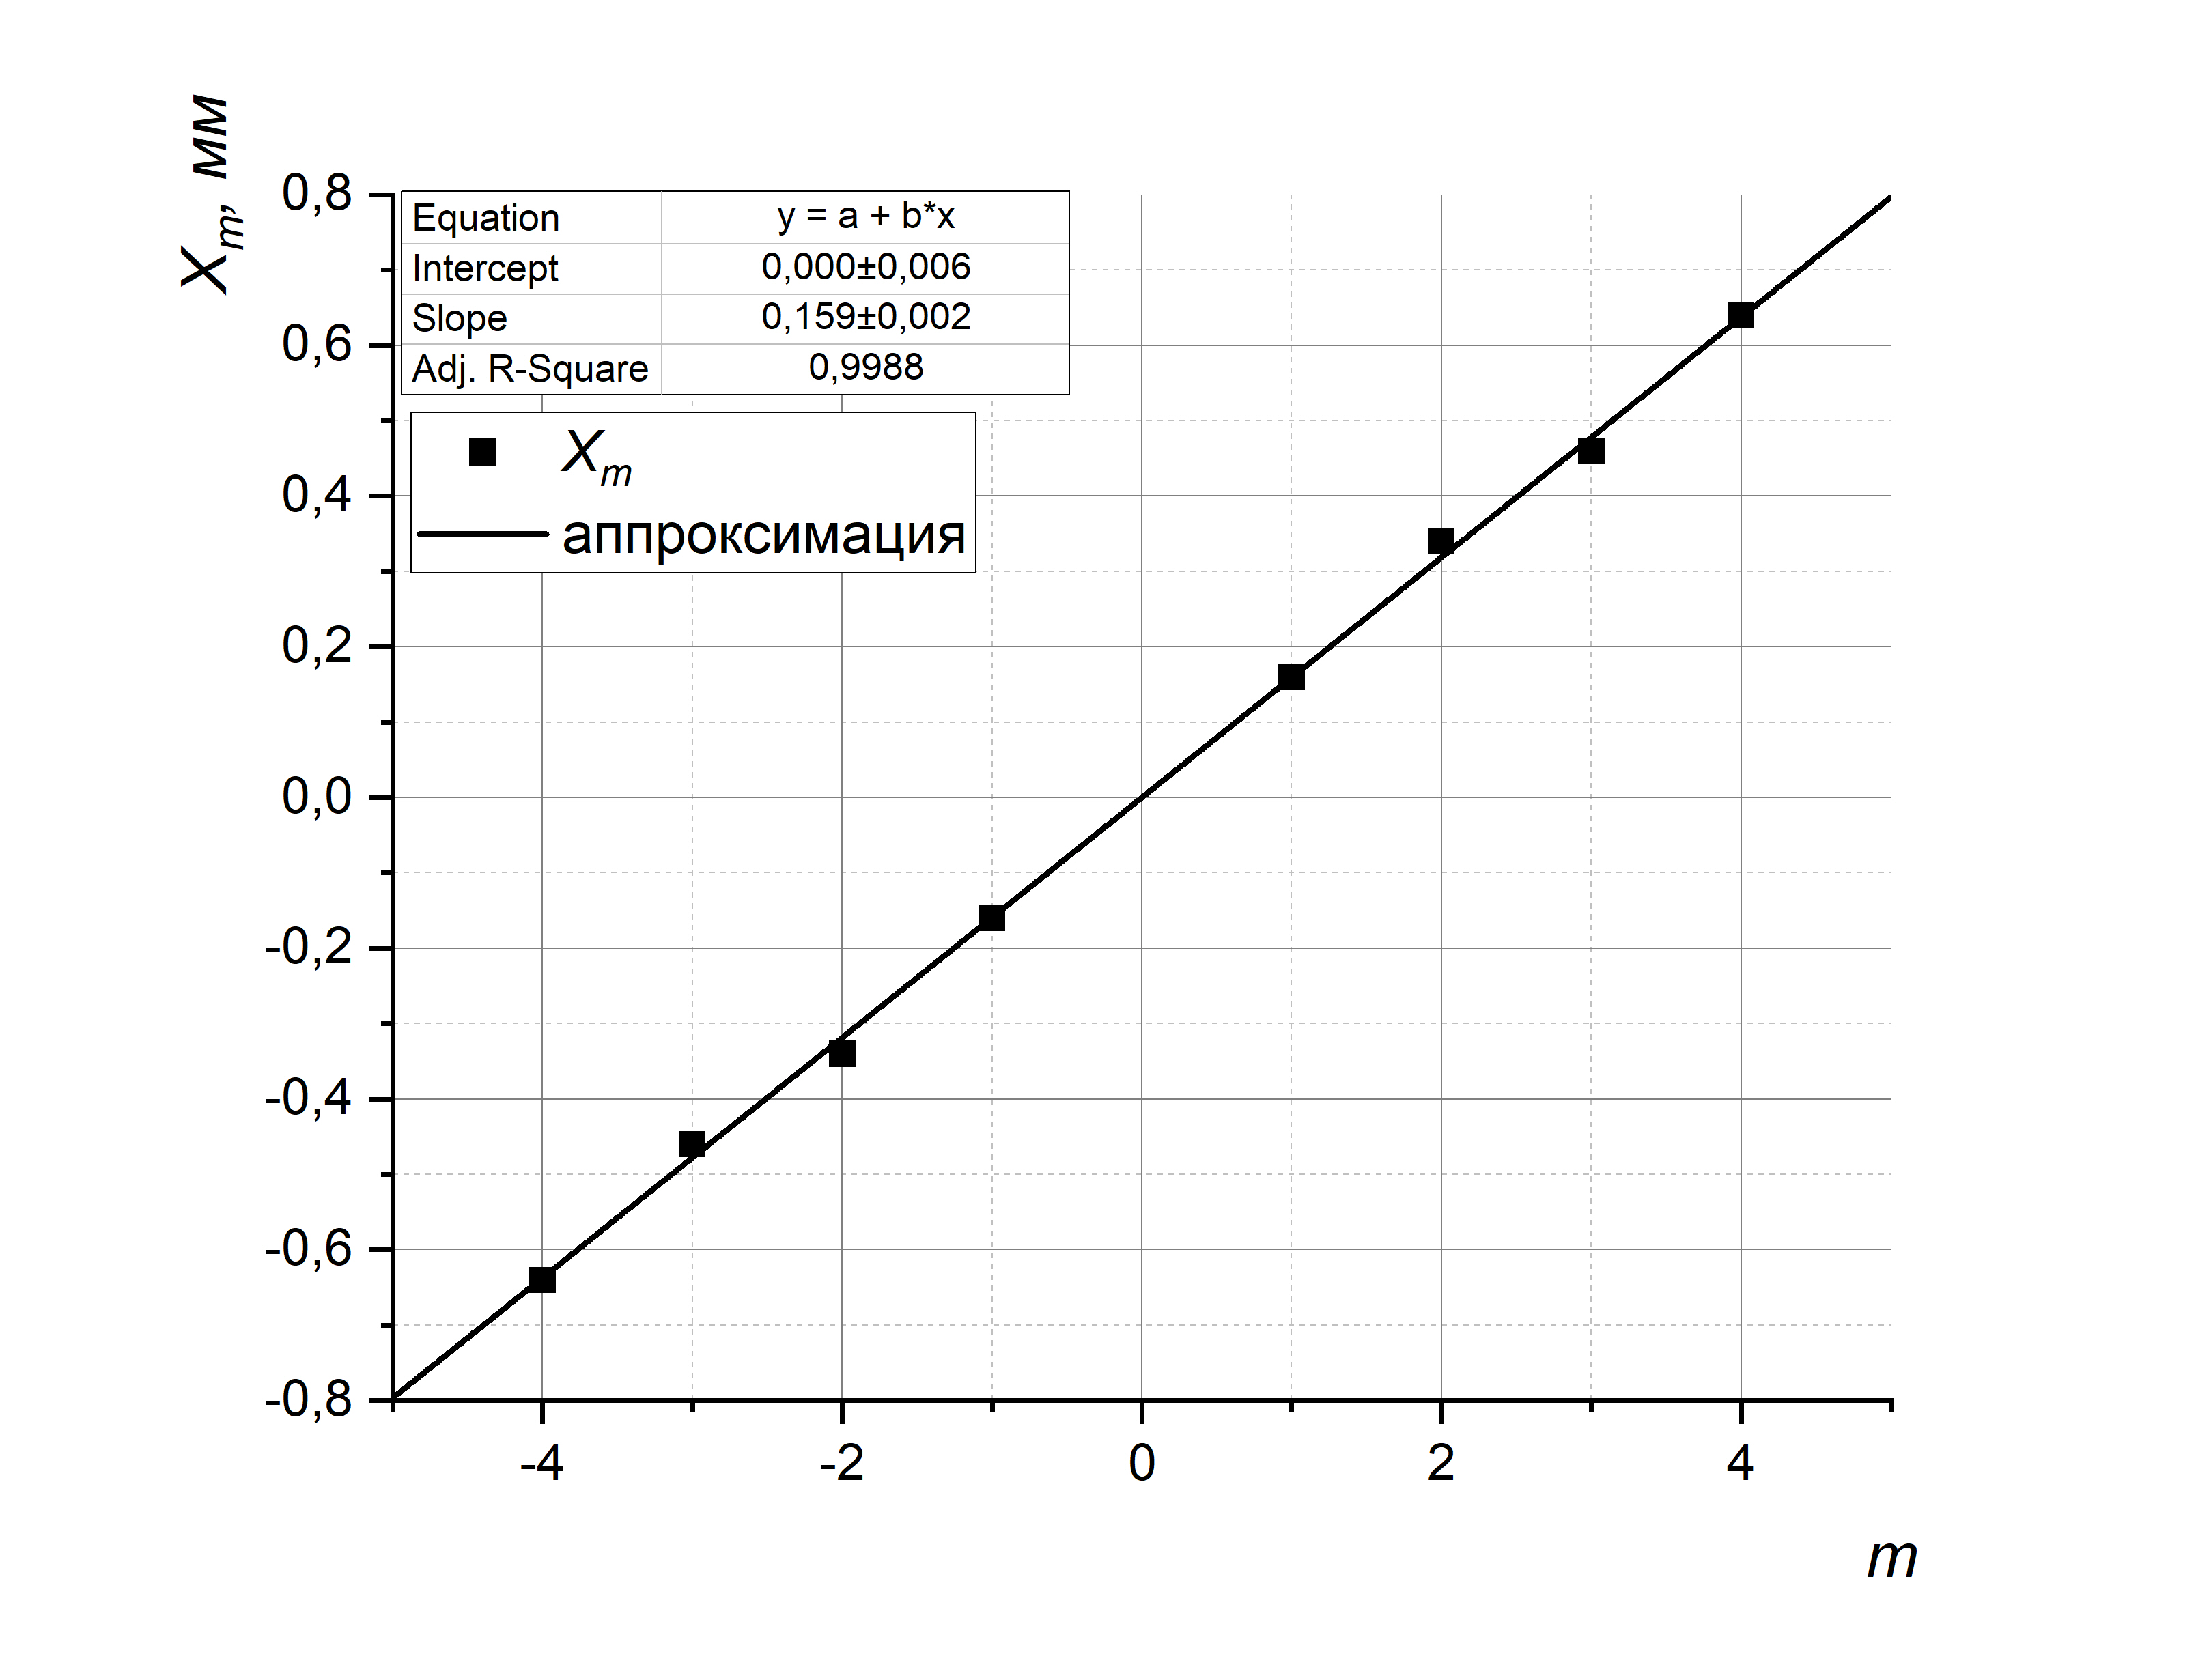
\includegraphics[width = 0.8\textwidth]{9.jpg}
\caption{Визуализация данных и аппроксимация}
\end{center}
\end{figure}

\item Поскольку наклон графика у нас получился $k = (0,159 \pm 0,002)$ мм. Отсюда $\Delta X = (0,159 \pm 0,002)$ мм.

Все числа и погрешности для наклона графика мы взяли из МНК, а именно 
\[k = \dfrac{\left<xy \right>}{\left<x^2\right>}, \sigma_k \approx \dfrac{1}{\sqrt{n}} \sqrt{\dfrac{\left<y^2\right>}{\left<x^2\right>} - k^2}\]
\item Убедимся, что смещение щели $S_2$ не приводит к сдвигу картины. 
\item При уменьшении щели масштаб картинки уменьшается, пока картинка полностью не исчезнет.
\end{enumerate}
\section{Дифракция Фраунгофера для двух щелей}
\subsection*{Установка}
Заменим $S_2$ на две щели 

\begin{figure}[h]
\begin{center}
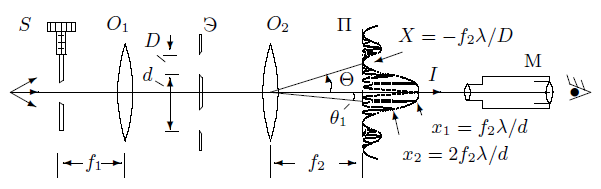
\includegraphics[width = 0.8\textwidth]{4.png}
\caption{Установка для третьего пункта}
\end{center}
\end{figure}

В этом случае легко видеть, что угловая координата максимума будет 
\begin{equation}
\theta_m = \frac{m \lambda}{d}
\end{equation}
И между соседними полосами 
\begin{equation}
\delta x = f_2 \frac{\lambda}{d}
\end{equation}
Так же нетрудно оценить число интерференционных полос укладывающихся в области центрального максимума 
\begin{equation}
n = \frac{2d}{D}
\end{equation}
\subsection*{Ход работы}
\begin{enumerate}
\item Не перемещая линз заменим $S_2$ и, слегка передвигая ее вдоль скамьи, найдем резкое изображение.
\item Определим расстояние между темными полосками внутри центрального максимума. Посчитаем число светлых промежутков между ними. Измерим ширину центрального максимума. $X = (0,720 \pm 0,005)$ мм, между ними $n = 11 \pm 1$ светлых промежутков.

Погрешность для $X$ взялась из половины цены деления, а для $n$ она появилась в связи с тем, что мы могли сбиться, при подсчете полос.
\item Далее определим расстояние $\delta x$ между минимумами по формуле $\delta x = \frac{X}{n} = (65 \pm 5)$ мкм. Далее из формулы $(9)$ мы можем получить расстояние $d$ между щелями
\[d = (0,97 \pm 0,05) \text{мм}\]

Здесь погрешность берется из формулы
\[\delta d = d \cdot \sqrt{\left(\dfrac{\partial \left(f_2 \frac{\lambda}{\delta x}  \right)}{\partial \left(\delta x\right)}\right)^{2} \cdot \sigma_{\delta x}^2} = d \cdot f_2\lambda \dfrac{1}{\delta x^2} \cdot \sigma_{\delta x}\]
В итоге, вспомнив и выражении для $d$ получаем, что 
\[\delta d = \dfrac{d^2}{\delta x} \sigma_{\delta x}\]
Измерив мы получили, что 
\[d = (1,000 \pm 0,005) \text{мм}\]
\[D = (0,180 \pm 0,005) \text{мм}\]

Погрешность берем как половину цены деления.
Отсюда из формулы $(10)$ мы получаем, что
\[n_{theor} = 11 \pm 1\]
Погрешность для $n$ берем из формулы 
\[\delta n = n \cdot \sqrt{\left(\dfrac{\partial \frac{2d}{D}}{\partial d}\right)^{2} \cdot \delta_{d}^2 + \left(\dfrac{\partial \frac{2d}{D}}{\partial D}\right)^{2} \cdot \delta_{D}^2} = \sqrt{\dfrac{4\delta_d^2}{D^2} + \dfrac{4d^2\delta_{D}^2}{D^4}}\]
\item Исследуем влияние когерентности на видность картины. Для этого расширяя щель $S$ подберём $b_0$ такую, при которой первый раз исчезают интерференционные полосы. $b_{0pract} = (0,0715 \pm 0,0005)$ мм. Из формулы 
\[\dfrac{b}{f_1} = \dfrac{\lambda}{d}\]
мы получаем, что 
\[b_{theor} = 0,060 \pm 0,002 \text{мм}\]
Погрешность для этой формулы опять таки берется из
\[\delta b = b \cdot \left|\dfrac{\partial \frac{f_1 \lambda}{d}}{\partial d}\right| \sigma_d = \dfrac{b f_1 \lambda}{d^2} \cdot \sigma_d = \dfrac{b^2\sigma_d}{d}\]
\end{enumerate}
\section{Влияние дифракции на разрешающую способность оптического инструмента}
\subsection*{Схема установки}

\begin{figure}[h]
\begin{center}
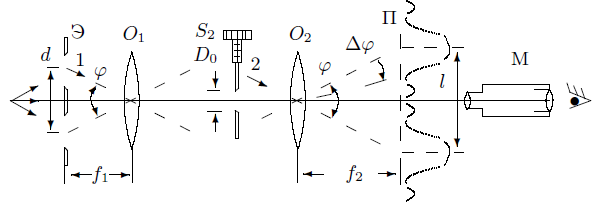
\includegraphics[width = 0.8\textwidth]{5.png}
\caption{Схема установки для пункта 4.}
\end{center}
\end{figure}

Если перед $O_2$ расположить $S_2$, то изображение объекта будет искажено из-за дифракции. Качественной характеристикой этого искажения может служить $\varphi_{min}$ --- минимальное угловое между объектами (источниками). 

\begin{equation}
\varphi = \frac{d}{f_1}
\end{equation}
Из геометрии $l$ между объектами равно 
\begin{equation}
l = \phi \cdot d_2
\end{equation}
\begin{equation}
\dfrac{\lambda}{D_0} = \dfrac{l}{f_2} = \dfrac{d}{f_1}
\end{equation}
\subsection*{Ход работы}
\begin{enumerate}
\item Собрать схему, изменив в схеме из предыдущего пункта только $S$.
\item Поставить между линзами щель $S_2$ и уменьшая ее ширину наблюдать ухудшение изображения. Подобрать ширину $S_2$ так, чтобы изображения почти сливались.
\[D_0 = (0,055 \pm 0,005)\text{мм}\]


Погрешность берем как половину цены деления.
В итоге получаем, что выполнено соотношение $(13)$.
\item Поставить двойную щель и измерить расстояние между щелями и толщину самих щелей. 
\[d = (1,000 \pm 0,005) \text{мм}\]
\[D = (0,180 \pm 0,005) \text{мм}\]

Погрешность берем как половину цены деления.
\end{enumerate}
\section*{Вывод}
Приведем итоги наших вычислений в таблице:

\begin{table}[h]
\begin{tabular}{|c|c|c|c|c|}
\hline
                & \begin{tabular}[c]{@{}c@{}}Дифракция \\ Френеля\end{tabular} & \begin{tabular}[c]{@{}c@{}}Дифракция \\ Фраунгофера\\ на одной щели\end{tabular} &                 & \begin{tabular}[c]{@{}c@{}}Дифракция \\ Фраунгофера\\ на двух щелях\end{tabular} \\ \hline
$D_{theor}$, мм & $0,28\pm 0,2$                                                          & $0,38 \pm 0,04$                                                                            & $d_{theor}$, мм & $0,97\pm0,05$                                                                             \\ \hline
$D_{prac}$, мм  & $0,285\pm 0,005$                                                        & $0,395\pm 0,005$                                                                            & $d_{prac}$, мм  & $1,000\pm0,005$                                                                             \\ \hline
\end{tabular}
\end{table}

Из нее мы видим, что все теоретические формулы, приведенные в данной работе хорошо сходятся с измерениями. 

Так же в работе были проверены и подтверждены качественные рассуждения.
\end{document}